\chapter{Large language models}


\begin{description}
    \item[Conditional generation] \marginnote{Conditional generation}
        Generate text conditioned on the input tokens (i.e., prompt).

        \begin{figure}[H]
            \centering
            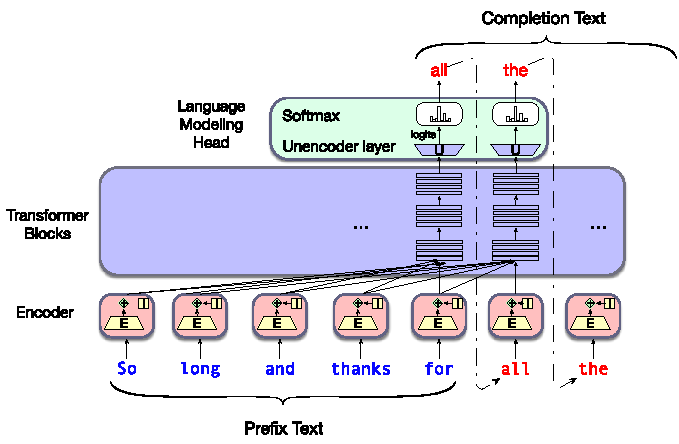
\includegraphics[width=0.45\linewidth]{./img/_conditional_generation.pdf}
        \end{figure}

        \begin{example}[Sentiment analysis]
            Given the prompt:
            \[ p = \texttt{the sentiment of the sentence `I like Jackie Chan' is} \]
            Determine the probability of the tokens \texttt{positive} and \texttt{negative}:
            \[
                \prob{\texttt{positive} \mid p} \qquad \prob{\texttt{negative} \mid p}
            \]
        \end{example}

        \begin{example}[Question answering]
            Given the prompt:
            \[ p = \texttt{Q: who wrote the book `The origin of Species'? A:} \]
            Determine the tokens of the answer autoregressively:
            \[
                \arg\max_{w_1} \prob{w_1 \mid p}, \arg\max_{w_2} \prob{w_2 \mid pw_1}, \dots
            \]
        \end{example}
\end{description}


\section{Decoding strategies}

\begin{description}
    \item[Greedy decoding] \marginnote{Greedy decoding}
        Select the next token as the most probable of the output distribution.

        \begin{remark}
            Greedy decoding risks getting stuck in a local optimum.

            \indenttbox
            \begin{example}
                Consider the following search tree of possible generated sequences:
                \begin{figure}[H]
                    \centering
                    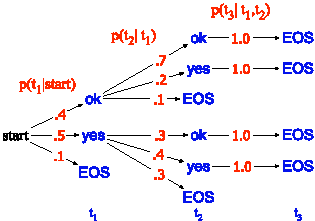
\includegraphics[width=0.3\linewidth]{./img/_greedy_decoding_local_minimum.pdf}
                \end{figure}

                Greedy search would select the sequence \texttt{yes yes} which has probability $0.5 \cdot 0.4 = 0.2$. However, the sequence \texttt{ok ok} has a higher probability of $0.4 \cdot 0.7 = 0.28$.
            \end{example}
        \end{remark}

    \item[Beam search] \marginnote{Beam search}
        Given a beam width $k$, perform a breadth-first search keeping at each branching level the top-$k$ tokens based on the probability of that sequence:
        \[ \log\left( \prob{y \mid x} \right) = \sum_{i=1}^{t} \log\left( \prob{ y_i \mid x, y_1, \dots, y_{i-1} } \right) \]

        \begin{example}
            Consider the following tree with beam width $k=2$:
            \begin{figure}[H]
                \centering
                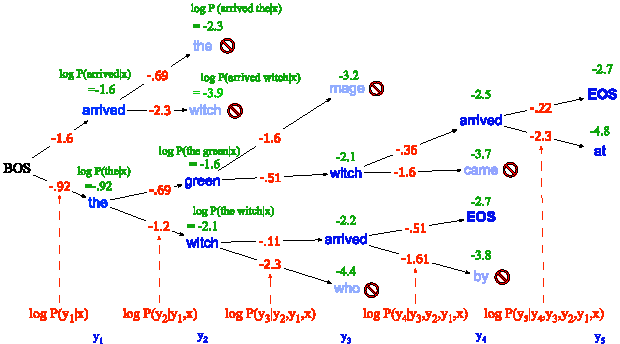
\includegraphics[width=0.7\linewidth]{./img/_beam_search.pdf}
            \end{figure}
            The selected sequence is \texttt{[BOS] the green witch arrived [EOS]}.
        \end{example}

        \begin{remark}
            As each path might generate sequences of different length, the score is usually normalized by the number of tokens as:
            \[ \log\left( \prob{y \mid x} \right) = \frac{1}{t} \sum_{i=1}^{t} \log\left( \prob{ y_i \mid x, y_1, \dots, y_{i-1} } \right) \]
        \end{remark}

        \begin{remark}
            The likelihood of the sequences generated using beam search is higher than using greedy decoding. However, beam search is still not optimal.
        \end{remark}

    \item[Sampling] \marginnote{Sampling}
        Sample the next token based on the output distribution.

        \begin{description}
            \item[Random sampling]
                Sample considering the distribution over the whole vocabulary.

                \begin{remark}
                    By adding-up all the low-probability words (which are most likely unreasonable as the next token), their actual chance of getting selected is relatively high.
                \end{remark}

            \item[Temperature sampling]
                Skew the distribution to emphasize the most likely words and decrease the probability of less likely words. Given the logits $\vec{u}$ and the temperature $\tau$, the output distribution $\vec{y}$ is determined as:
                \[ \vec{y} = \texttt{softmax}\left( \frac{\vec{u}}{\tau} \right) \]
                where:
                \begin{itemize}
                    \item Higher temperatures (i.e., $\tau > 1$) allow for considering low-probability words.
                    \item Lower temperatures (i.e., $\tau \in (0, 1]$) focus on high-probability words.
                    \begin{remark}
                        A temperature of $\tau = 0$ corresponds to greedy decoding.
                    \end{remark}
                \end{itemize}


            \item[Top-k sampling]
                Consider the top-$k$ most probable words and apply random sampling on their normalized distribution.

                \begin{remark}
                    $k=1$ corresponds to greedy decoding.
                \end{remark}

                \begin{remark}
                    $k$ is fixed and does not account for the shape of the distribution.
                \end{remark}

            \item[Top-p sampling]
                Consider the most likely words such that their probability mass adds up to $p$. Then, apply random sampling on their normalized distribution.
        \end{description}
\end{description}